% J. Gudmundsson, J. Katajainen, D. Merrick, C. Ong, and T. Wolle, “Compressing spatio-temporal trajectories,” Computa- tional Geometry, vol. 42, no. 9, pp. 825–841, 2009.
% PRESS
% REST!!!
% SQUISH?
% GML?
% Douglas pecker
% Dead Reckoning
\section{Douglas-Peucker}
\textcite{dp} introduced the Douglas-Peucker (DP) line simplification algorithm. It is a Top-Down algorithm, which means it recursively partitions the line until some halting condition is met, from \cite{Sun2016}. DP begins by removing all points except for the end points, then it adds the point furthest from the line back into the graph. As this happens the line is updated to go through the newly added point. This process continues recursively by adding the point farthest from the line and updating the line until no point is further away than a certain threshold. See an example iteration of DP in figure \ref{dp}. The halting condition is met when no point is a further than the distance $d$ from the line.

DP's worst case runtime is $O(n^{2})$, however it is still used for its simplicity and efficiency in practice \cite{gudmundsson2009compressing}. Additionally, \textcite{gudmundsson2009compressing}, created an improved version which can run in $O(n\log(n))$ even in if the path is polygonal and self intersects. There are also implementations of DP that use spatio-temporal distance measures like SED.
\begin{figure}[h]
    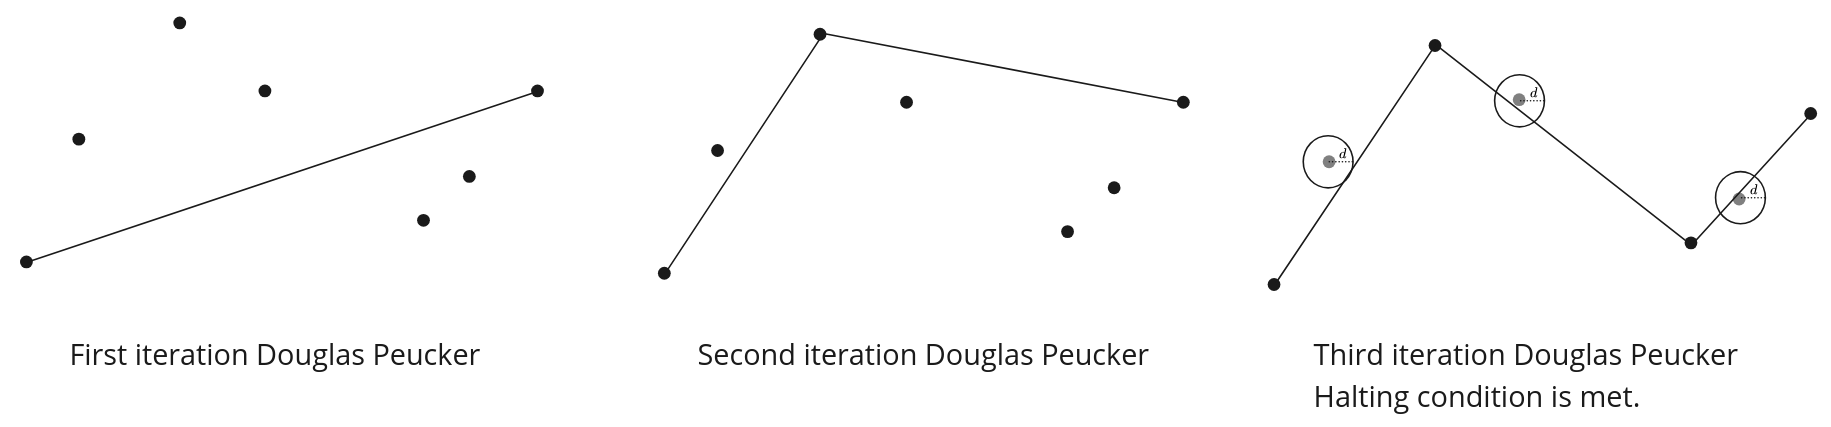
\includegraphics[width=1.0\linewidth]{./figures/dp.png}
    \caption{Three iteration of the Douglas Peucker algorithm, where the halting condition is met in the third iteration.}
    \label{dp}
\end{figure}

\section{SQUISH and SQUISH-E}
\textcite{muckell2011squish} introduced the Spatial QUalIty Simplification heuristic (SQUISH). It is a simple algorithm based on buffers and SED estimation. An input variable $\beta$ defines the buffer size. The algorithm sequentially loops through all the points in the trajectory; points are added to the buffer until it is filled. When a point is added the locally estimated SED error that would be introduced if the point is removed is calculated.

The first point is given an estimation of positive infinity, as it cannot be removed. When a point is added and the buffer is full, the point with the lowest estimated introduction of error is removed. This point is also referred to as the point with the highest priority. The introduction of error for its neighbors is then re-estimated. The neighbors contain some hidden information about the point that was removed, therefore the re-estimation will increase their estimated introduction of error. This process continues by removing the highest priority point in the buffer until all points have been processed. The result is a buffer filled with the points that represent the compressed trajectory. This algorithm has a run-time complexity of $O(n\log{\beta})$. It is important to note that the buffer size is static and defined as an input variable, which leads to predictable memory usage during execution.

In figure \ref{fig:squish} an example of the algorithm with a buffer size 4 is shown. The buffer is gradually filled up with points and their estimated introduction of error. When the buffer is full and point $E$ is processed, the highest priority point $B$ is removed. After removal, point $E$ is added and the error is re-estimated for $B$'s neighbors $A$ and $C$.

While this algorithm performs well compared to others when considering SED for small compression ratios, it has severe drawbacks such as the local estimations' incapability with large compression ratios. As a result, \textcite{muckell2014compression} introduced Spatial QUalIty Simplification Heuristic Extended (SQUISH-E), an improved version of the original algorithm.

\begin{wrapfigure}[23]{r}{0.5\textwidth}
    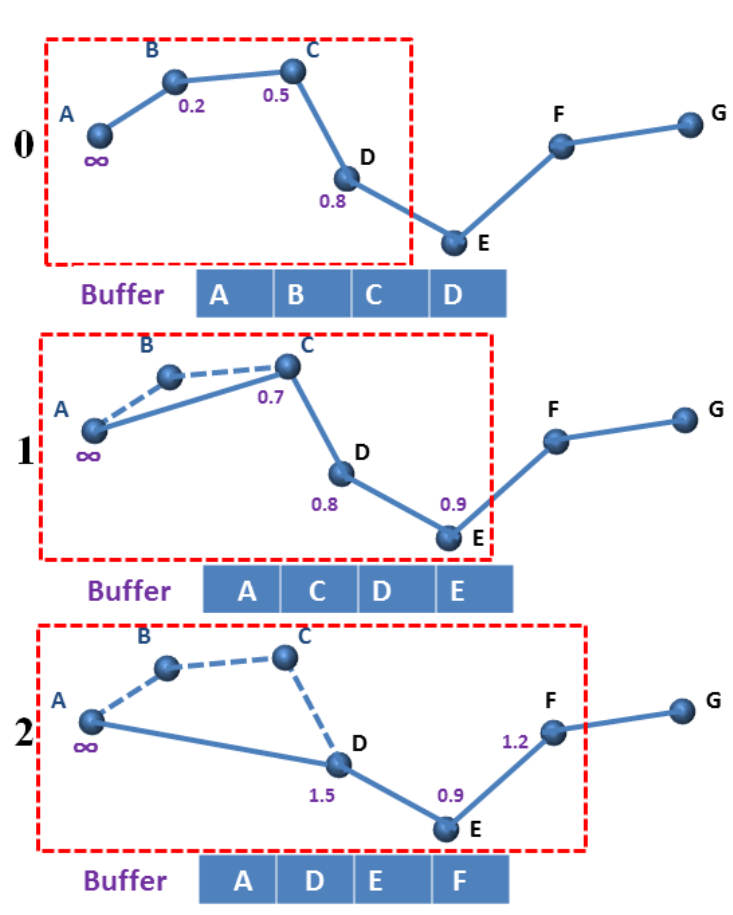
\includegraphics[width=0.5\textwidth]{./figures/squish.png}
    \caption{SQUISH estimates the lowest SED error
        and removes the point which is predicted to introduce
        the lowest amount of error into the compression. From, \cite{muckell2011squish}.}
    \label{fig:squish}
\end{wrapfigure}

The central change in SQUISH-E is a flexible buffer size combined with a maximum SED threshold. This change ensures that no point with an estimated SED over a certain threshold is removed, instead the buffer is expanded. The improved algorithm introduces two additional parameters: $\lambda$ and $\mu$. $\lambda$ represents the target compression ratio and $\mu$ represents the upper limit for SED error. Using these parameters, two modes are defined: SQUISH-E($\lambda$) and SQUISH-E($\mu$). In SQUISH-E($\lambda$), $\mu$ is set to zero, causing the algorithm to minimize SED error while ensuring a compression ratio of $\lambda$. On the other hand, SQUISH-E($\mu$) refers to the situation where $\lambda$ is set to 1. This will maximize the compression ratio while keeping SED error below $\mu$.

Experimental results from \textcite{muckell2014compression}, show that SQUISH-E provides low SED errors with a much faster run time than any of the alternatives. Additionally, the algorithm allows for control over both compression ratio and accuracy, providing flexibility that is not offered by other algorithms.

\section{PRESS}
\textcite{song2014press}, introduced the novel framework PRESS (\underline{P}aralleled \underline{R}oad-Network-Based Trajectory Compre\underline{ss}ion). PRESS compresses trajectories from road networks efficiently, using three key features to achieve this. Firstly it separates the spatial path and the temporal information when representing a trajectory. Secondly it introduces a lossless spatial compression algorithm called Hybrid Spatial Compression (HSC). Thirdly PRESS supports many common queries for location based services without decompression.

The reason to separate spatial and temporal information is to better exploit the road network in compression, this is essential for the HSC algorithm. HSC first compresses based on shortest paths. It has a map of all shortest paths from node $e_i$ to $e_j$, if the trajectory to compress is exactly like the shortest path from $e_i$ to $e_j$, it simply stores these nodes instead of the spatial information in the trajectories. This strategy is employed based on the assumption that people will often take the shortest path when traveling in a road network. Afterwards HSC compresses based on frequent sub-trajectory (FST) coding. It will represent the remaining trajectories as FST codes, giving the most frequent FSTs the shortest codes. This way huge amounts of space is saved, since a code is significantly smaller than a trajectory. In additional PRESS implements the Bounded Temporal Compression (BTC) algorithm. BTC tries to remove nodes from the trajectory without creating large temporal errors. To measure the error, two error metrics are used; Time Synchronous Network Distance (TSND) and Network Synchronous Time Distance (NSTD). TSND is the maximum distance between a trajectory $T$ and its compressed version $T'$. NSTD is the maximum time difference between a trajectory $T$ and its compressed version $T'$, see figure \ref{press_error}. The result is lossless spatial compression and bounded temporal compression, ensuring high quality compressed data.

\begin{figure}[t]
    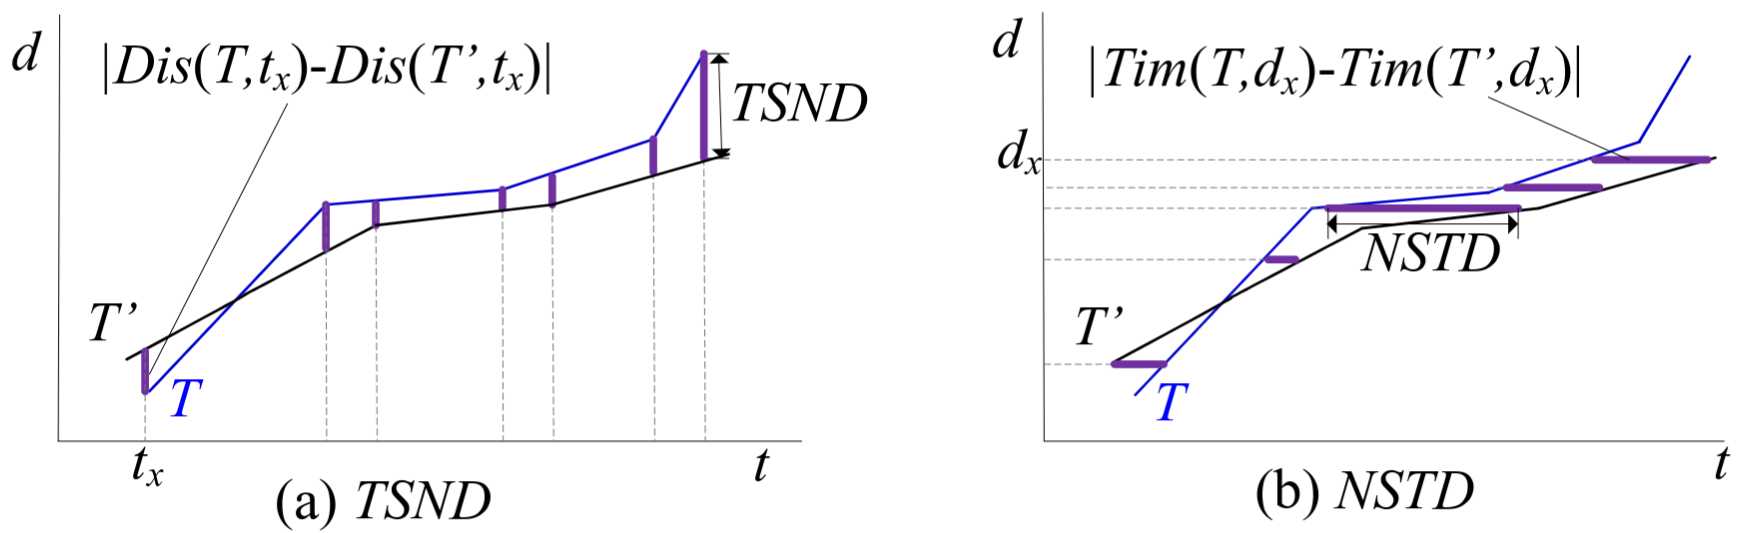
\includegraphics[width=1.0\linewidth]{./figures/press_error.png}
    \caption{TSND and NSTD, from \cite{song2014press}.}
    \label{press_error}
\end{figure}

The experimental results show that PRESS outperforms many competitors drastically in terms of compression ratio. PRESS was compared against two state-of-the-art approaches for trajectory compression in road networks. Map-matched trajectory compression (MMTCS) and Nonmaterial. When considering compression ratio we also need to define the error metric (aka, TSND and NSTD). With TSND and NSTD equal to 0, meaning no error tolerance, PRESS improved MMTC's compression ratio by 64\% and Nonmaterial's by 43\%. For TSED = 600 m, PRESS improved MMCTC's compression ratio by 280\% and Nonmaterial's by 199\%. These results show a significant improvement for compression ratio by a novel method.

\textcite{han2017compress} made a further improved version of PRESS called, COMPRESS (\underline{Com}prehensive \underline{P}aralleled \underline{R}oad-Network-Based Trajectory Compre\underline{ss}ion). This replaced the HSC part of PRESS with Hybrid Dictionary Compression (HDC) and Labeling and Coding (L\&C). COMPRESS is very similar to PRESS, but has multiple algorithms optimized for different data-types. Which makes it more applicable to multiple use cases.



\section{REST}
\label{sec:REST}
\textcite{zhao2018rest} introduced the REST (\underline{Re}ference-based \underline{S}patio-\underline{t}emporal trajectory compression) framework, which aims to efficiently represent raw trajectories by generating reference trajectories. The REST framework is categorized as bounded lossy compression. The objective is to minimize the error of the compression while using as few reference trajectories as possible. This approach is data driven, as it directly uses the raw trajectories to create the reference trajectory set.  Prior to REST, the only available data-driven method was PRESS. \textcite{zhao2018rest} mention some drawbacks of PRESS as motivation for creating the framework. One limitation of PRESS is that it limits trajectories to originate from a known road network. This can be problematic as there exists a large amount of unconstrained geospatial data. In addition, the algorithm needs updated road networks, which can be problematic due to frequent changes. However, REST has some similarities with PRESS in that reference trajectories are very similar to the frequent sub-trajectories (FSTs) in PRESS. The key difference is that reference trajectories in REST are unconstrained and data driven. While the FSTs in PRESS are partly data driven and constrained to a road network. This allows REST to be more easily generalized.

\begin{wrapfigure}[13]{r}{0.5\textwidth}
    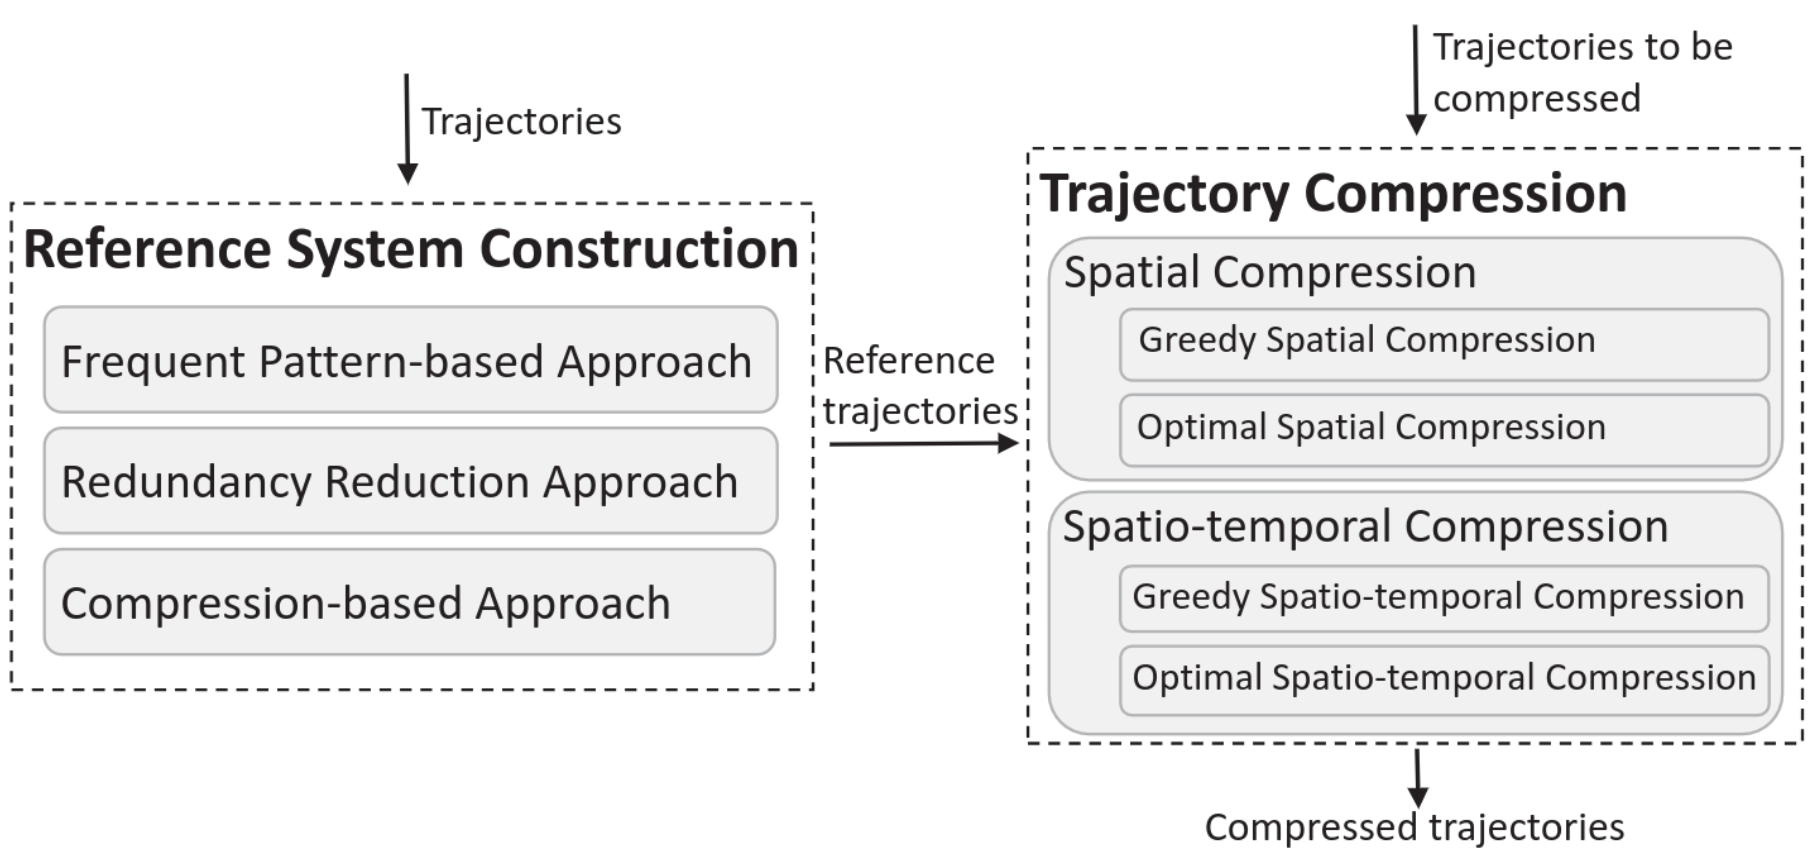
\includegraphics[width=0.5\textwidth]{./figures/rest_structure.png}
    \caption{REST framework overview, from \cite{zhao2018rest}.}
    \label{fig:rest_overview}
\end{wrapfigure}

Another motivation for creating REST was that existing trajectory compression frameworks like SQUISH, do not effectively utilize the characteristics of the entire trajectory set. SQUISH compresses trajectories individually in a vacuum, without considering their similarities. \textcite{zhao2018rest} also criticized SQUISH for assuming that moving objects do not frequently change speed and direction while traveling, which does not accurately represent real-world behavior. Consequently, algorithms like this cannot achieve high compression rates on real-world data. In contrast, data-driven compression such as REST, does not require such assumptions.

The structure of REST consists of two parts: the reference system construction and the compression of raw trajectories using the reference set, as seen in figure \ref*{fig:rest_overview}. Three methods were created for reference system construction; Frequent Pattern-based analysis, Redundancy reduction approach, and Compression-based approach. The methods attempt to create reference sets with high coverage and low redundancy. For the compression strategy, different methods were implemented in the categories spatial-only/spatio-temporal and greedy/optimal. Greedy Spatial Compression (GSC), Optimal Spatial Compression (OSC), Greedy Spatio-Temporal Compression (GSTC), and Optimal Spatio-Temporal Compression (OSTC). The greedy algorithms optimize locally instead of globally, therefore they are faster but with less accuracy than the optimal algorithms. The spatial-only algorithms only consider the spatial aspect which is simpler than the spatio-temporal aspect, they are both faster and more accurate (for spatial accuracy metrics).

From the experimental results, it was concluded that the Compression-based approach (CA) was the most effective. This approach compress training trajectories with the existing reference set and uses the compression ratio to interpret wheteher the training trajectory is reduntant or not. A high compression ratio indicates that the trajectory is redundant and should not be added to the reference set, a low compression ratio, on the other hand, indicates that the trajectory is not redundant and should be added to the reference set.

\begin{wrapfigure}[19]{r}{0.5\textwidth}
    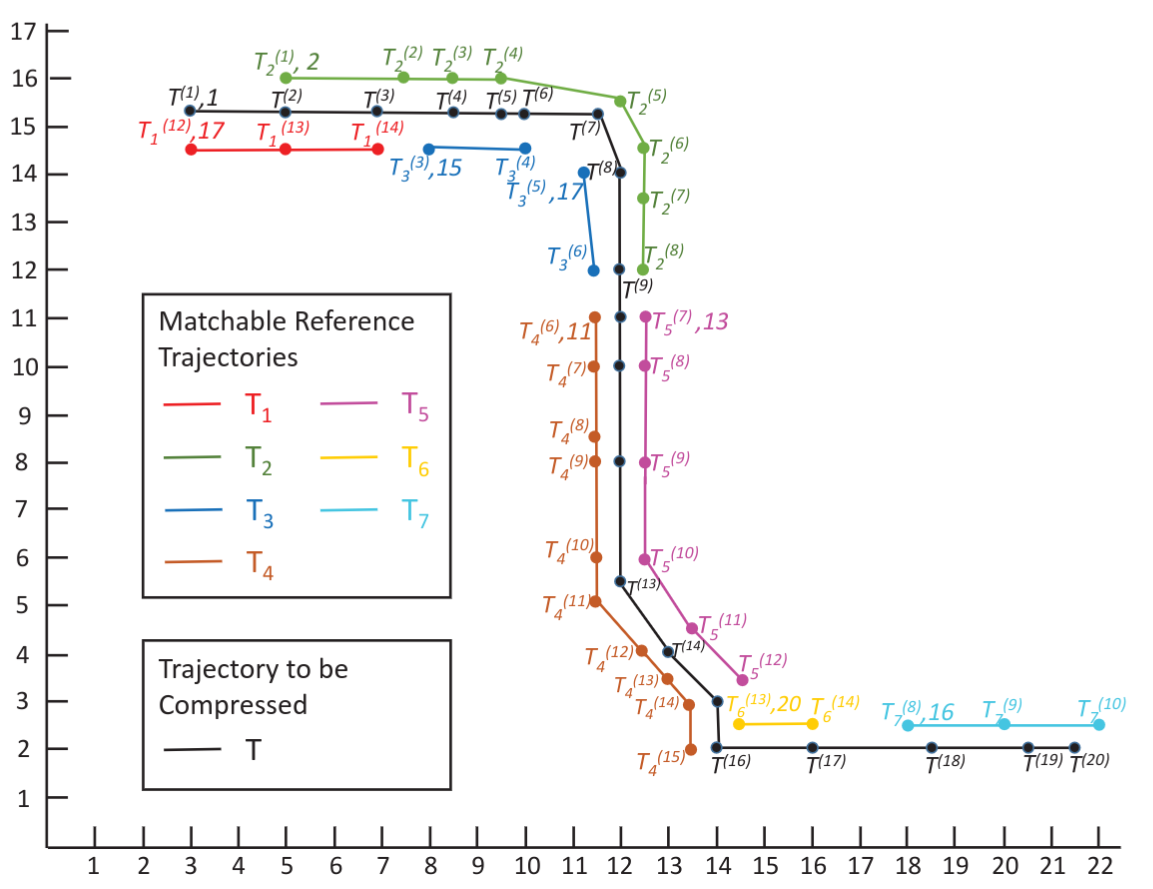
\includegraphics[width=0.5\textwidth]{./figures/rest.png}
    \caption{Matchable Reference Trajectories, from \cite{zhao2018rest}.}
    \label{fig:rest}
\end{wrapfigure}

In terms of trajectory compression, the results show that GSTC is preferred because it was the most well rounded algorithm. It was second most efficient (second to Douglas Peucker) and second to OSTC in accuracy. GSTC iteratively replaces the longest sub-trajectory with its Matchable Reference Trajectory (MRT). When selecting reference trajectory, GSTC selects the MRT that results in the lowest time correction cost. The time correction cost is defined as a variation of DTW, called MaxDTW. MaxDTW is different from DTW in that it looks at the maximum DTW across all pairs instead of the sum. In the figure \ref{fig:rest}, first $T^{(1,3)}$ is replaced by $T_1^{(12,14)}$, then $T^{(4,9)}$ is replaced by $T_2^{(3,8)}$, then $T^{(10,16)}$ is replaced by $T_4^{(6,15)}$, then $T^{(17)}$ remains in the compressed trajectory. The final segment $T^{(18,20)}$ is replaced by $T_7^{(8,10)}$

The results show that REST outperforms existing methods like PRESS and Douglas Peucker in terms of compression ratio and efficiency. One advantage of REST is that it is more flexible than existing methods, as it can be used in both constrained and non-constrained spaces. REST is also able to compress trajectories in spatial-only and spatio-temporal domains. The reference set can be stored using a much smaller storage space, as it is only a subset of all trajectories. Lastly the compressed data is simply a sequence of reference trajectories. This means that the compressed data is indexable and usable without computing any decompressed version. However, some memory lookup must be performed to retrieve the referenced trajectoryies. An index structure for this has not been implemented yet and is mentioned as future work.

